\documentclass[tikz,border=10pt]{standalone}
\usepackage{amsmath}
\usepackage{tikz}
\begin{document}
	
	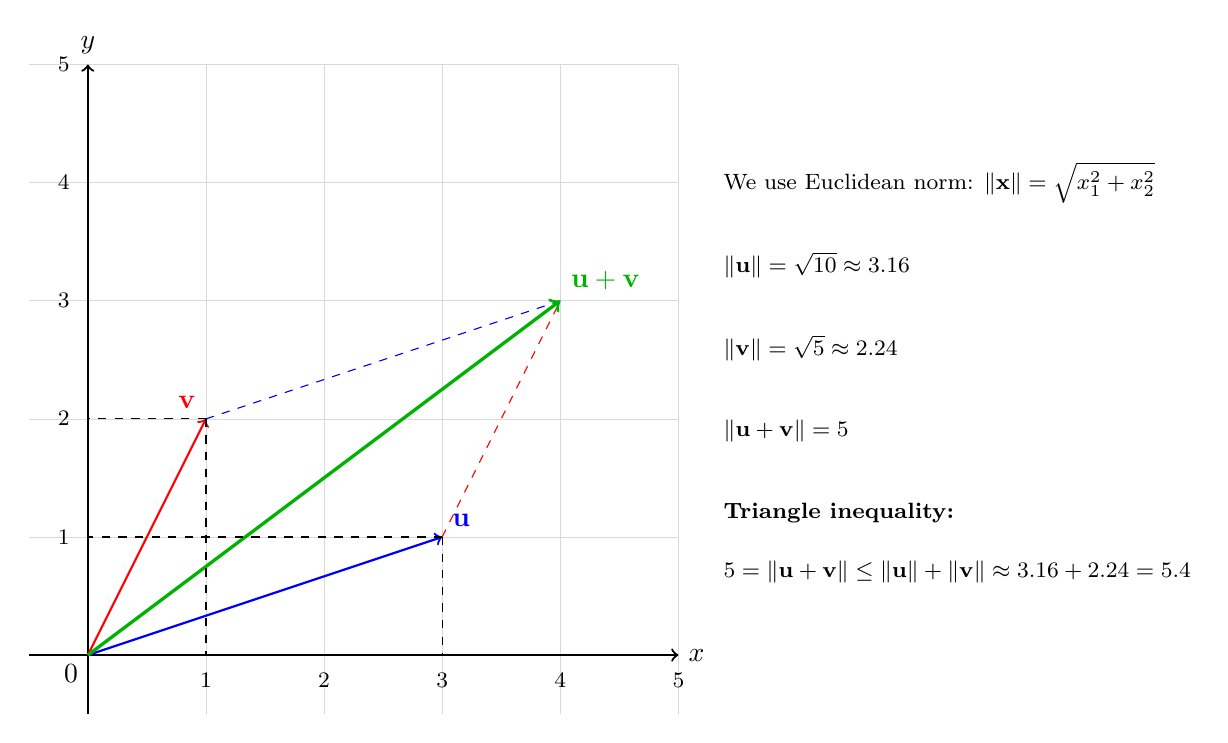
\begin{tikzpicture}[scale=1.5]
		
		\draw[very thin, gray!30] (-0.5,-0.5) grid (5,5);
		\draw[->, thick] (-0.5,0) -- (5,0) node[right] {$x$};
		\draw[->, thick] (0,-0.5) -- (0,5) node[above] {$y$};
		
		\foreach \x in {1,2,3,4,5} 
		\draw (\x,0) node[below=3pt] {\footnotesize $\x$};
		
		\foreach \y in {1,2,3,4,5} 
		\draw (0,\y) node[left=3pt] {\footnotesize $\y$};
		
		\node at (0,0) [below left] {$0$};
		
		\draw[->, thick, blue] (0,0) -- (3,1) node[above right] {$\mathbf{u}$};
		\draw[->, thick, red] (0,0) -- (1,2) node[above left] {$\mathbf{v}$};
		
		\draw[dashed, red] (3,1) -- (4,3);
		\draw[dashed, blue] (1,2) -- (4,3);
		
		\draw[->, very thick, green!70!black] (0,0) -- (4,3) node[above right] {$\mathbf{u} + \mathbf{v}$};
		
		\draw[dashed, black] (3,1) -- (3,0);
		\draw[dashed, black] (3,1) -- (0,1);
		
		\draw[dashed, black] (1,2) -- (1,0);
		\draw[dashed, black] (1,2) -- (0,2);
		
		\node[black, right] at (5.3,4) {\footnotesize We use Euclidean norm: $\|\mathbf{x}\| = \sqrt{x_1^2 + x_2^2}$};
		\node[black, right] at (5.3,3.3) {\footnotesize $\|\mathbf{u}\| = \sqrt{10} \approx 3.16$};
		\node[black, right] at (5.3,2.6) {\footnotesize $\|\mathbf{v}\| = \sqrt{5} \approx 2.24$};
		\node[black, right] at (5.3,1.9) {\footnotesize $\|\mathbf{u} + \mathbf{v}\| = 5$};
		\node[black, right] at (5.3,1.2) {\footnotesize \textbf{Triangle inequality:}};
		\node[black, right] at (5.3,0.7) {\footnotesize $5 = \|\mathbf{u} + \mathbf{v}\| \leq \|\mathbf{u}\| + \|\mathbf{v}\| \approx 3.16 + 2.24 = 5.4$};
		
	\end{tikzpicture}
	
\end{document}
